\documentclass[a4paper,12pt]{report}
\usepackage[catalan]{varioref}
\usepackage{setspace}
\usepackage[margin=2.54cm]{geometry}
\usepackage{pdfpages}
\usepackage[utf8]{inputenc}
\usepackage[catalan]{babel}
\usepackage{graphicx,subcaption}
\usepackage{graphics}
\usepackage{lscape}
\usepackage{pdflscape}
\usepackage{float}
\usepackage{textcomp}
\usepackage{amsmath}
\usepackage{hyperref}
\usepackage{subcaption}
\usepackage{pgfplots}
\usepackage{tikz}
\usepackage{fancyvrb}
\usepackage{parskip}
\usepackage{changepage}
\usepackage{enumitem}
\usepackage{tcolorbox}
\usepackage[all]{hypcap}
\usepackage{xcolor}
\usepackage{listings}
\definecolor{green}{HTML}{228B22}
\definecolor{orange}{HTML}{FFC107}
\usepackage{color}
\definecolor{dkgreen}{rgb}{0,0.6,0}
\definecolor{gray}{rgb}{0.5,0.5,0.5}
\definecolor{mauve}{rgb}{0.58,0,0.82}
\lstset{escapeinside={<@}{@>}}

\hypersetup{
    colorlinks,
    citecolor=black,
    filecolor=black,
    linkcolor=black,
    urlcolor=blue
}


\lstset{frame=tb,
    language=python,
    aboveskip=3mm,
    belowskip=3mm,
    showstringspaces=false,
    columns=flexible,
    basicstyle={\small\ttfamily},
    numbers=none,
    numberstyle=\tiny\color{gray},
    keywordstyle=\color{blue},
    commentstyle=\color{dkgreen},
    stringstyle=\color{mauve},
    breaklines=true,
    breakatwhitespace=true, tabsize=3
}
\title{
	\begin{center}
	\vspace{3cm}
	
\includegraphics[width=11cm, height=3cm]{images/Logo-uoc.png}
	\end{center}
	\begin{center}
	\line(1,0){400}
	\end{center}		
	TIPOLOGIA I CICLE DE VIDA DE LES DADES\\
	\vspace{2mm}
	\Large PAC1: Què son les dades i quin el seu cicle de vida?\\
	\line(1,0){400}
	\vspace{2.5cm}
	}

\author{Marc Cervera Rosell \vspace{1cm}}


\date{Semestre: febrer 2025 - juny 2025\vspace{0.5cm} \\ Màster en ciència de dades}
\onehalfspacing

\begin{document}
\thispagestyle{empty}
	\begin{titlepage}
		\maketitle
		\thispagestyle{empty}
	\end{titlepage}
	\cleardoublepage
	\newpage

\thispagestyle{empty}
\tableofcontents
\thispagestyle{empty}
\listoffigures
\thispagestyle{empty}
\newpage
\pagenumbering{arabic}
%\thispagestyle{empty}
\section*{Exercici 1}
\addcontentsline{toc}{section}{Exercici 1}
\subsection*{Pregunta 1}
\addcontentsline{toc}{subsection}{Pregunta 1}
Per aplicar la tècnica de normalització caldria, en primer lloc, seleccionar aquelles variables numèriques a les quals volem aplicar la tècnica i després ajustar-les a una escala més reduïda, per tal de, fer-les més comprensibles. Típicament, les escales són entre -1.0 i 1.0 o entre 0.0 i 1.0.\\
Per aplicar la tècnica de discretització cal, com en el cas anterior, seleccionar aquelles variables numèriques a les quals volem aplicar la tècnica. Seguidament, cal substituir els valors numèrics per una sèrie d'etiquetes les quals poden ser conceptuals o intervals. Aquesta tècnica permet consolidar un possible criteri d'agrupació de dades. Per exemple, un \textit{dataset} amb els resultats dels balanços d'empreses. Es podria substituir els resultats dels balanços per 'positiu', 'negatiu' i 'neutre' i, posteriorment, agrupar pel resultat del balanç.\\
Aquestes tècniques són molt importants per als models de predicció, ja que permeten que les dades siguin més senzilles d'interpretar i això comporta que el rendiment del model sigui millor i que aquest tingui la capacitat de trobar patrons més fàcilment, és a dir, el model es fa més senzill.
\subsection*{Pregunta 2}
\addcontentsline{toc}{subsection}{Pregunta 2}
Mentre un enginyer de dades treballa en el desenvolupament, construcció, prova i manteniment d'arquitectures, un científic de dades és una persona que es dedica a obtenir informació rellevant sobre les dades, a partir de preguntes que s'ha plantejat, i a transmetre aquesta informació de manera senzilla. A més, tot i que ambdós perfils tenen coneixements de programació, l'enginyer de dades no aprofundeix tant en coneixements d'estadística i matemàtiques com el científic de dades.\\
\href{https://www.linkedin.com/jobs/search/?currentJobId=4167044480&geoId=104738515&keywords=data%20scientist&origin=JOB_SEARCH_PAGE_SEARCH_BUTTON&refresh=true}{\underline{Oferta de \textit{data scientist}}}\\
\href{https://www.linkedin.com/jobs/search/?currentJobId=4172639382&geoId=104738515&keywords=data%20engineer&origin=JOB_SEARCH_PAGE_SEARCH_BUTTON&refresh=true}{\underline{Oferta de \textit{data engineer}}}
\subsection*{Pregunta 3}
\addcontentsline{toc}{subsection}{Pregunta 3}
Les set tasques que permeten un major nivell d'abstracció en la visualització de dades són:
\begin{itemize}
    \item Panorama general $\rightarrow$ Permet una visió de totes de les dades.
    \item Acostament $\rightarrow$ Permet focalitzar un punt concret de les dades.
    \item Filtratge $\rightarrow$ Permet filtrar els elements que no són d'interès.
    \item Detalls a petició $\rightarrow$ Permet obtenir detalls de les dades.
    \item Relacions $\rightarrow$ Permet veure com es relacionen les dades.
    \item Historial $\rightarrow$ Permet revisar/repetir versions anteriors.
    \item Extracció $\rightarrow$ Permet l'extracció de parts de les dades i els seus detalls.
\end{itemize}
\begin{figure}[H]
    \centering
    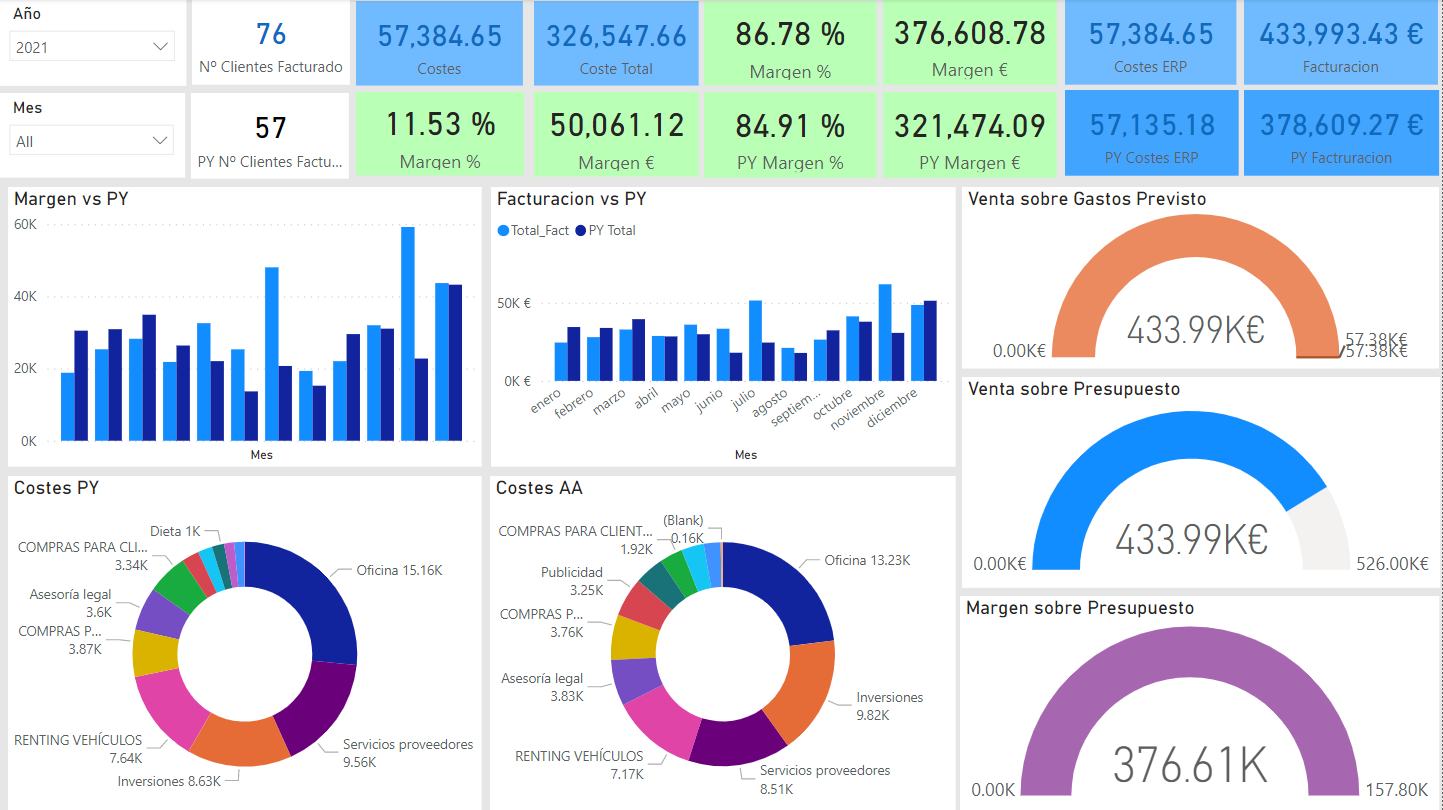
\includegraphics[scale = 0.2]{images/dashboard_ventas.png}
    \caption{Exemple de la tasca 'Panorama general'}
    \label{fig:panorama_general}
\end{figure}
\begin{figure}[H]
    \centering
    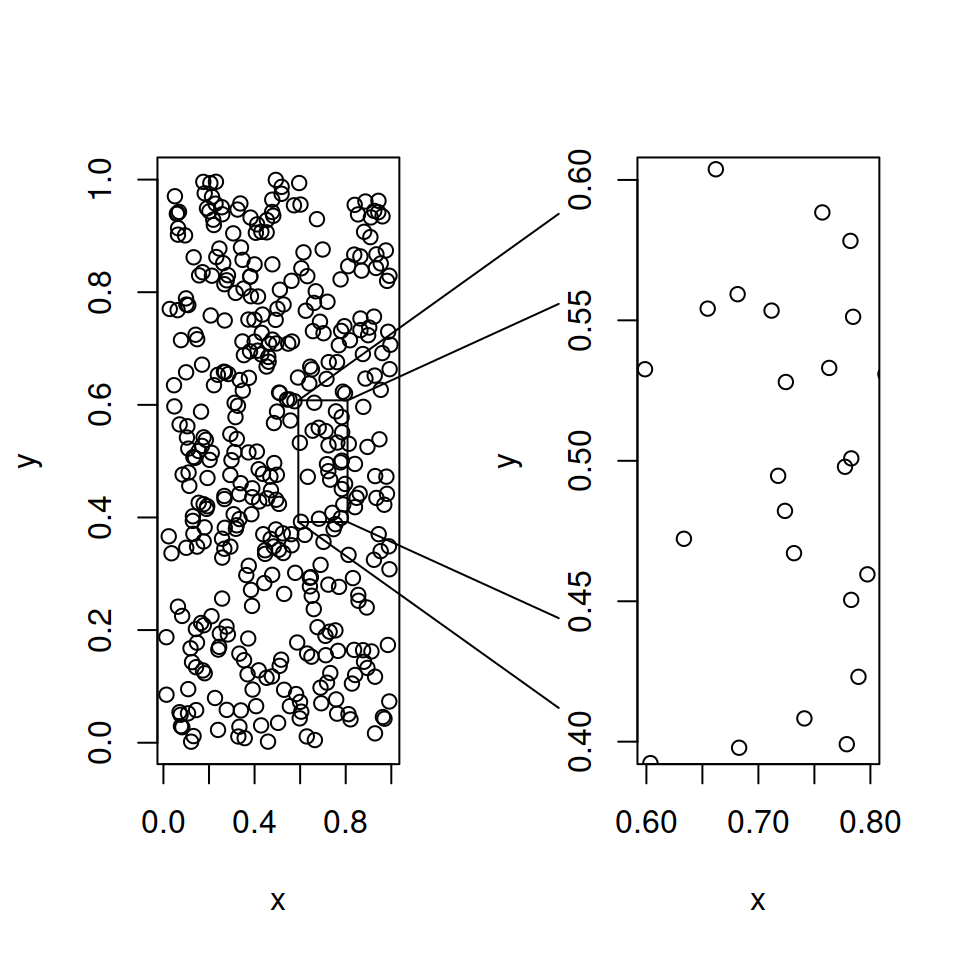
\includegraphics[scale = 0.8]{images/zoom.png}
    \caption{Exemple de la tasca 'Zoom'}
    \label{fig:zoom}
\end{figure}
\begin{figure}
    \centering
    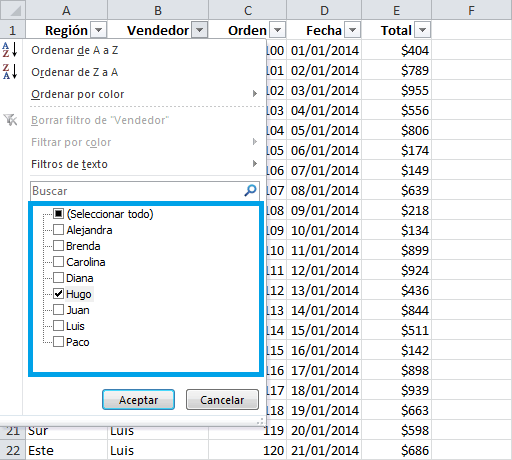
\includegraphics[scale = 0.7]{images/filtro.png}
    \caption{Exemple de la tasca 'Filtratge'}
    \label{fig:filtratge}
\end{figure}
\begin{figure}
    \centering
    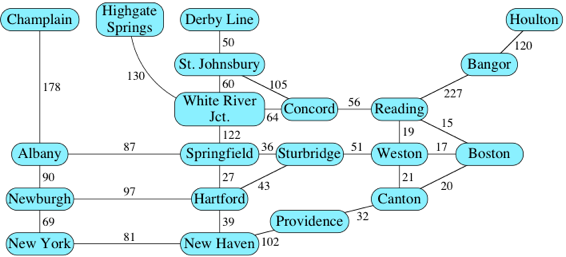
\includegraphics[scale =1.3]{images/8aa21944eef2879cea9080a2ae2fbcb98cec0ddf.png}
    \caption{Exemple de la tasca 'Relcions'}
    \label{fig:relacions}
\end{figure}
\newpage
\subsection*{Pregunta 4}
\addcontentsline{toc}{subsection}{Pregunta 4}
La primera etapa és la captura, que té com a objectiu la recol·lecció de les dades que es generen en un procés. Un exemple d'aquesta etapa podria ser, les dades d'un sensor IoT que recol·lecta un broker de Kafka.\\
La segona etapa és l'emmagatzematge i té com a objectiu guardar les dades capturades en bases de dades o fitxers en un format adequat per a la posterior explotació. L'exemple en aquest cas, seria l'emmagatzemament de les lectures del sensor IoT en una base de dades.\\
La tercera etapa és el preprocessament i té com a objectiu preparar les dades per la seva posterior anàlisi i explotació. L'exemple podria ser la neteja de les dades.\\
La quarta etapa és l'anàlisi, que té com a objectiu crear models per explicar les dades. L'exemple seria construir un model de predicció de falles del sensor IoT.\\
La penúltima etapa és la visualització que té com a objectiu presentar les dades. L'exemple seria un panell de PowerBI.\\
Finalment, la publicació, que documenta els resultats. L'exemple seria la redacció d'un \textit{report} amb els resultats obtinguts.
\subsection*{Pregunta 5}
\addcontentsline{toc}{subsection}{Pregunta 5}
La millor opció per a un sistema de monitoratge ambiental basat en sensors seria una base de dades no relacional a causa del fet que els sensors poden generar dades molt diverses. És a dir els sensors poden generar dades de tipus text, numèriques, imatges, so, etc. Per tant, considerant aquesta gran varietat que deriva en diferents esquemes per cada sensor es considera una millor opció una base de dades no relacional gràcies a la seva flexibilitat amb els esquemes de les dades i els seus tipus. A més, cal destacar que aquest tipus de bases de dades tenen un rendiment alt de lectura i escriptura. Per tant, en el sistema que es planteja, que captura volums de dades molt grans, és important poder consultar i inserir dades de la manera més ràpida possible. Finalment, un altre motiu pel qual una base de dades NoSQL és una millor opció és la capacitat d'escalar horitzontalment. És a dir, la capacitat d'afegir més recursos per a poder treballar amb volums de dades majors que en les bases de dades relacionals.
\subsection*{Pregunta 6}
\addcontentsline{toc}{subsection}{Pregunta 6}
La primera llibreria és \href{https://pandas.pydata.org/docs/}{\underline{Pandas}}. Les seves funcionalitats clau són la lectura i escriptura de dades, la manipulació de dades, el tractament de \textit{nulls}, l'agrupació, fusió i combinació i el tractament i anàlisi de \textit{time series}. Aquesta llibreria conté una funció per eliminar duplicats (\href{https://pandas.pydata.org/docs/reference/api/pandas.DataFrame.drop_duplicates.html}{\underline{\textit{drop\_duplicates()}}}), una funció que es pot usar per a corregir errates tipogràfiques, tot i que no està dissenyada específicament per això(\href{https://pandas.pydata.org/docs/reference/api/pandas.DataFrame.replace.html}{\underline{\textit{replace()}}}) i una funció per a la conversió de formats (\href{https://pandas.pydata.org/docs/reference/api/pandas.DataFrame.astype.html}{\underline{\textit{astype()}}}).
La segona eina és \href{https://pyjanitor-devs.github.io/pyjanitor/}{\underline{PyJanitor}}. És una llibreria basada en Pandas, per tant, les seves funcionalitats se centren simplificar algunes operacions de Pandas. Per eliminar duplicats es pot utilitzar la funció \textit{remove\_na()}. Per corregir errors tipogràfics i transformar formats, aquesta llibreria, no implementa cap funcionalitat especifia. En conseqüència, aquestes dues operacions s'haurien de realitzar amb Pandas o amb terceres llibreries.
\section*{Exercici 2}
\addcontentsline{toc}{section}{Exercici 2}
\subsection*{Pregunta 1}
\addcontentsline{toc}{subsection}{Pregunta 1}
Abans de procedir amb el \textit{web scraping}, caldrà tenir en compte que la violació de les normes de \textit{robots.txt}, pot comportar l'infringiment dels \textit{termes d'ús}. També, cal considerar la legislació vigent. En el cas del nostre país, el Regne d'Espanya, cal revisar dues lleis; la de propietat intel·lectual (\href{https://www.boe.es/buscar/pdf/1996/BOE-A-1996-8930-consolidado.pdf}{\underline{\textit{Real Decreto Legislativo 1/1996 de 12 de abril}}}) i la de protecció de dades personals i garantia de drets digitals (\href{https://www.boe.es/buscar/pdf/2018/BOE-A-2018-16673-consolidado.pdf}{\underline{\textit{Ley orgáica 3/2018 de 5 de diciembre}}}). Èticament, cal respectar la 'sagrada' voluntat del propietari de la \textit{web}, per això la millor manera de no infringir les normes del lloc \textit{web} i evitar incórrer en problemes legals és sol·licitar un permís per escrit del propietari on es demani consentiment per accedir a les dades. 

\section*{Bibliografia}
\addcontentsline{toc}{section}{Bibliografia}
\begin{itemize}
    \item \href{https://evotic.es/wp-content/uploads/2022/10/dashboard_ventas.png}{\underline{Imatge de l'exemple de 'Panorama general'}}
    \item \href{https://r-charts.com/es/correlacion/zoom-grafico_files/figure-html/zoom.png}{\underline{Imatge de l'exemple de 'Zoom'}}
    \item \href{https://cdn.exceltotal.com/wp-content/uploads/2014/02/filtros-en-excel-03.png}{\underline{Imatge de l'exemple de 'Filtratge'}}
    \item \href{https://cdn.kastatic.org/ka-perseus-images/8aa21944eef2879cea9080a2ae2fbcb98cec0ddf.png}{\underline{Imatge de l'exemple de 'Relacions'}}
    \item \href{https://www.arsys.es/blog/bases-de-datos-nosql-que-son-tipos-y-ventajas#tree-3}{\underline{Informació Bases de dades NoSQL}}
    \item \href{https://iddigitalschool.com/bootcamps/que-es-pandas/#:~:text=Funcionalidades%20Clave,filtrar%2C%20agregar%20y%20resumir%20datos.}{\underline{Pandas: La Herramienta Esencial para Data Science en Python}}
    \item \href{https://www.analyticslane.com/2021/07/15/pandas-cambiar-los-tipos-de-datos-en-los-dataframes/}{\underline{Pandas: Cambiar los tipos de datos en los DataFrames}}
    \item \href{https://hevodata.com/learn/guide-to-effective-data-cleaning-tools-in-python/#:~:text=1.-,Pandas,your%20data%20for%20further%20exploration.}{\underline{\textit{Most Helpful Data Cleaning Tools in Python for 2025}}}
\end{itemize}

\end{document}
